\documentclass[]{article}
\usepackage[formats]{listings}
\usepackage{graphicx}
\usepackage{amsmath}
\usepackage{slashed}


\usepackage{hyperref}
\hypersetup{
	colorlinks=true,
	linkcolor=blue,
	filecolor=magenta,      
	urlcolor=cyan,
	pdftitle={Sharelatex Example},
	bookmarks=true,
}

\lstdefineformat{R}{~=\( \sim \)}
\lstset{basicstyle=\ttfamily,format=R}

\title{aMC@NLO exam}
\author{Marco Rossi}

\begin{document}

\maketitle

\section{Day}

\subsection{$e^+ e^- \rightarrow q \bar{q}$}
\begin{figure}[b!]
	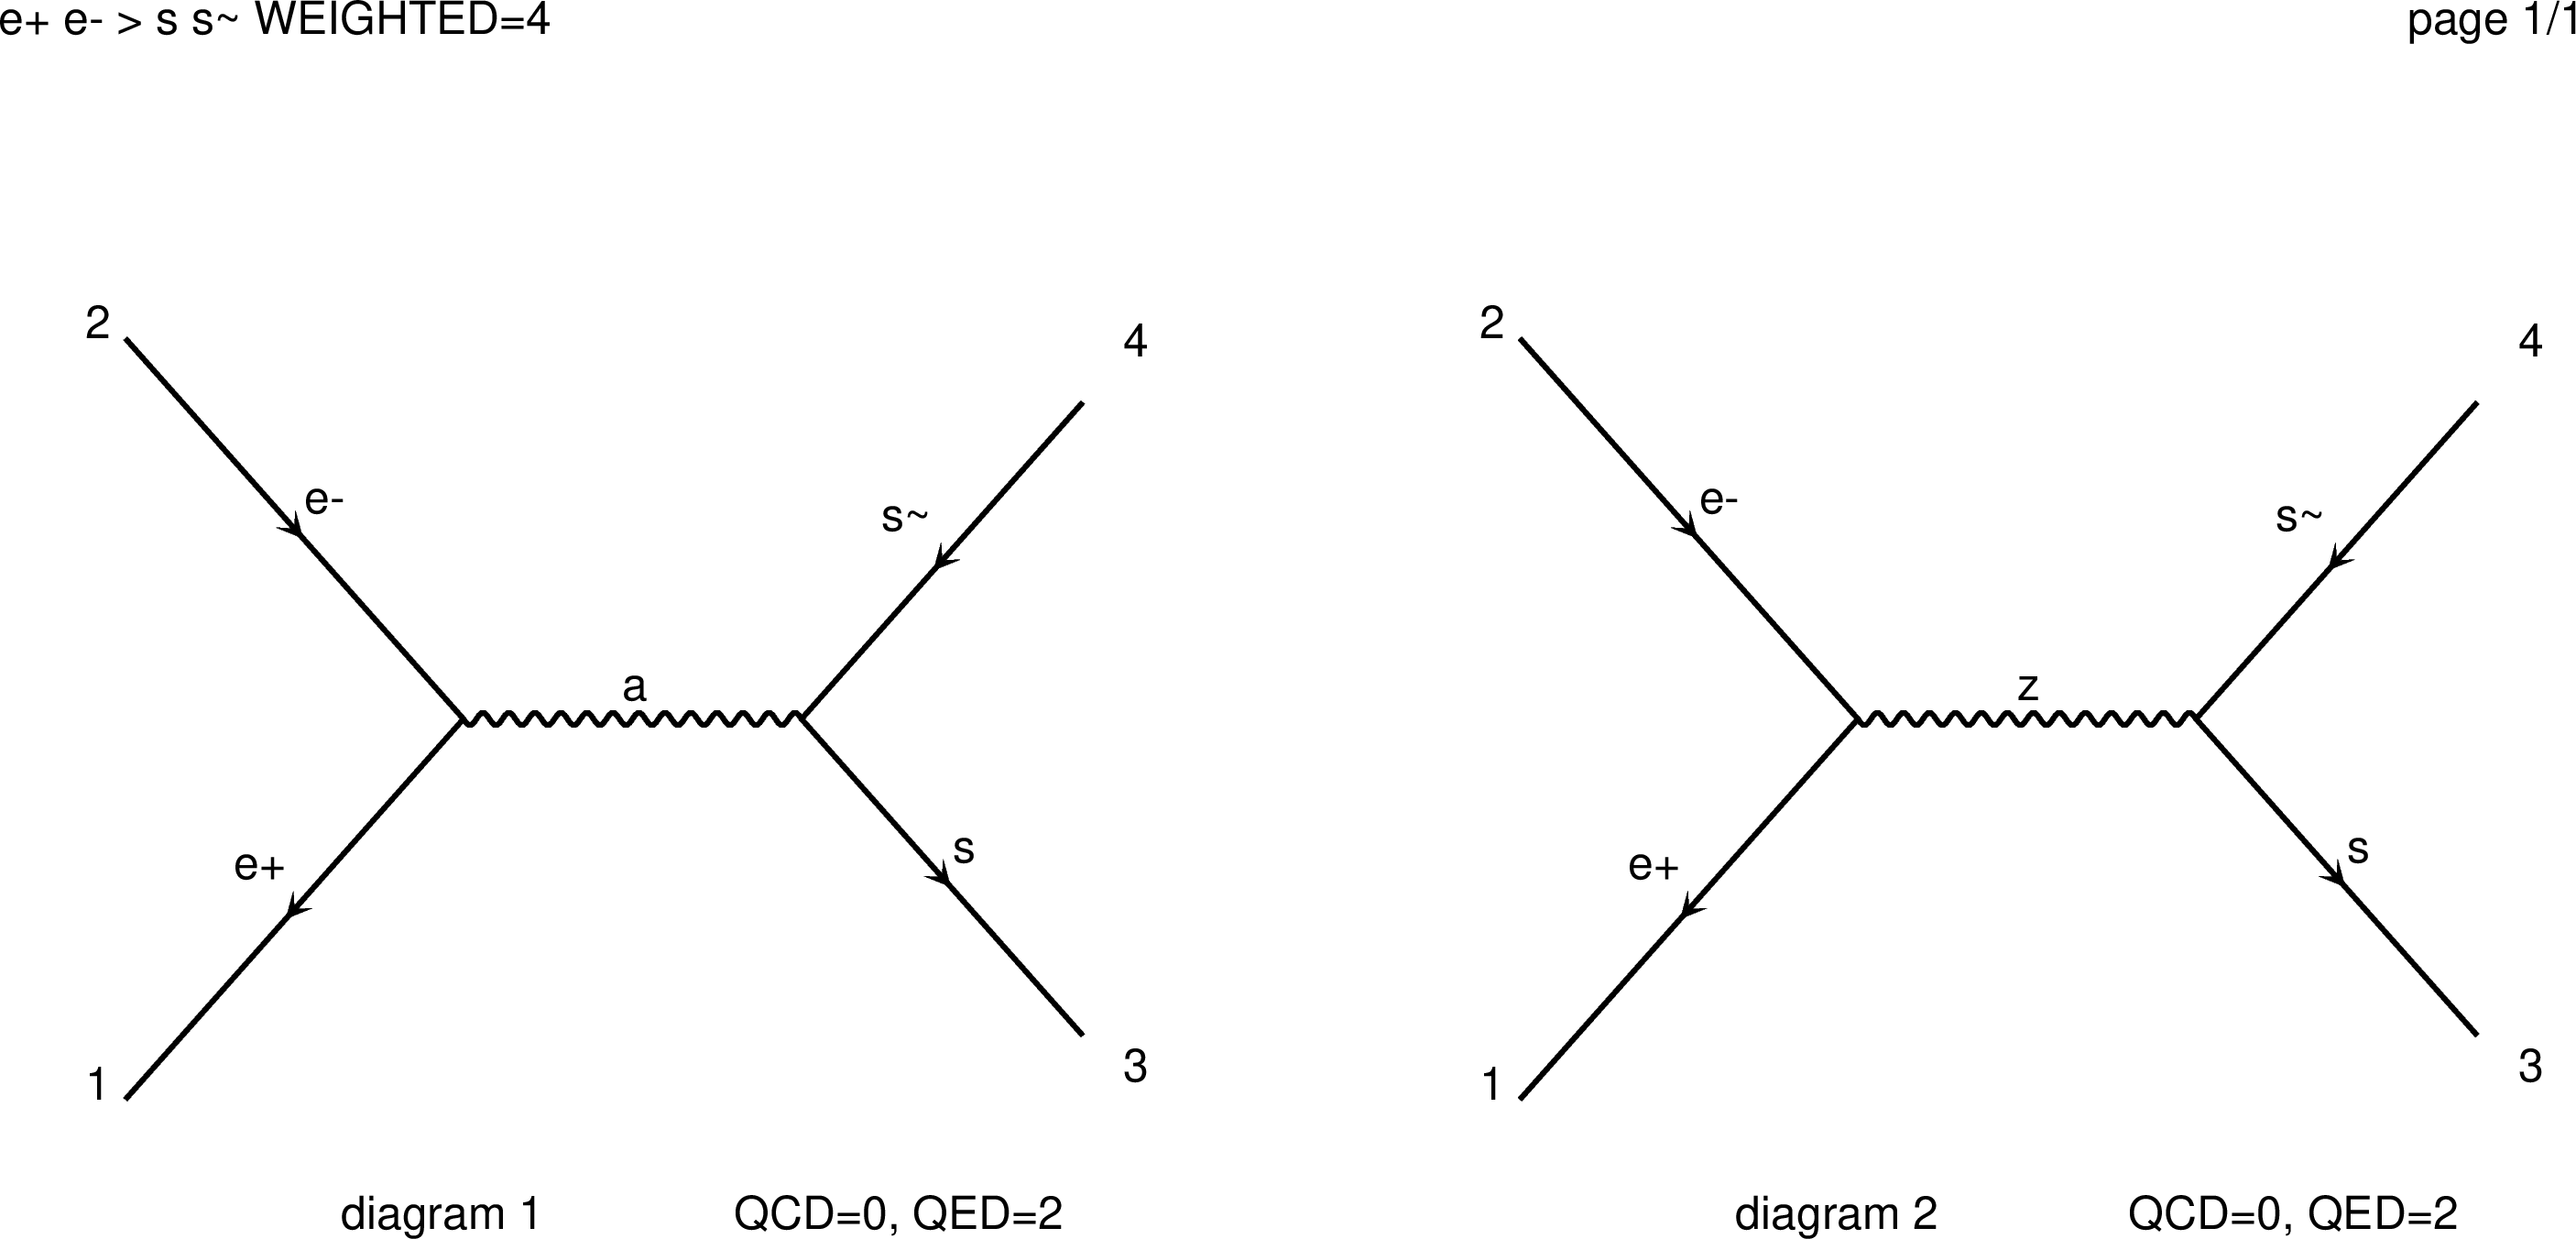
\includegraphics[width=\textwidth]{plots/diagrams.png}
	\caption{Leading order diagrams contributing to the $e^+ e^- \rightarrow q
	\bar{q}$ process.}
	\label{diagrams}
\end{figure}

Consider diagrams in fig.~\ref{diagrams}. The differential cross section of a
$2\rightarrow 2$ process is given by:
\begin{equation}
\label{xsec}
d\sigma = \frac{d\Phi_2}{4F} |\overline{\mathcal{M}}|^2
\end{equation}
The flux factor in the massless limit is simply $F=p_1\cdot p_2$, while the
differential phase space is:
\begin{equation}
	d\Phi_2=\frac{d^3\mathbf{p_3}}{(2\pi)^3 2E_3}\frac{d^3\mathbf{p_4}}{(2\pi)^32E_4}\,
	(2 \pi)^4\,\delta^{(4)}(p_1+p_2-p_3-p_4) = \frac{d \cos\theta}{16 \pi}
\end{equation}
Define the Mandelstam variables:
\begin{equation}
s = (p_1+p_2)^2 \qquad t = (p_1-p_3)^2 \qquad u = (p_1-p_4)^2
\end{equation}
such as $s+t+u=0$ in the massless limit.
The differential cross section can be written as:
\begin{equation}
\label{diff-xsec}
d\sigma = \frac{d\,\cos\theta}{32\pi \,s} |\overline{\mathcal{M}}|^2
\end{equation}
where a factor $2\pi$ arises from the integration over the azimuthal angle
$\varphi$, since matrix elements do not depend upon it.

\subsubsection{$e^+ e^- \rightarrow \gamma^* \rightarrow q \bar{q}$}
The amplitude for the process $e^+ e^-$ into $q \bar{q}$, mediated by a photon,
$\gamma$ is:
\begin{equation}
	\mathcal{M}_\gamma = 4 \pi i \alpha Q_f \bar{v}(p_1)\gamma^\mu u(p_2)\,
	\frac{g_{\mu\nu}}{q^2}\,\bar{u}(p_3)\gamma^\nu v(p_4)
\end{equation}
where $q = p_1+p_2$, so that $s=q^2$.
Then, after summing over the final state polarizations, averaging over the initial
ones and adding the color factor (the photon is color blind), the matrix element
squared is:
\begin{equation}
	|\overline{\mathcal{M}_\gamma}|^2 = N_c\frac{(4\pi\alpha Q_f)^2}{4s^2}
	\mathrm{Tr}\big[\slashed{p}_1 \gamma^\mu \slashed{p}_2 \gamma^\nu\big]
	\mathrm{Tr}\big[\slashed{p}_3 \gamma_\mu \slashed{p}_4 \gamma_\nu\big]
\end{equation}
This is possible because for Dirac massless spinors, the sum over polarizations
formulae hold:
\begin{equation}
\sum_r \bar{u}_r(p) u_r(p) = \slashed{p} \qquad\sum_r \bar{v}_r(p) v_r(p) = \slashed{p}
\end{equation}
Now, compute the traces over Dirac matrices with the help of the following identity:
\begin{equation}
\mathrm{Tr}[\gamma^\mu \gamma^\nu \gamma^\rho \gamma^\sigma] =
4(\eta^{\mu\nu}\eta^{\rho\sigma}-\eta^{\mu\rho}\eta^{\nu\sigma}+
\eta^{\mu\sigma}\eta^{\nu\rho})
\end{equation}
where $\eta^{\mu\nu}$ is the Minkowski metric tensor.
The trace in the four dimensional space is:
\begin{equation}
\mathrm{Tr}[\slashed{p}_1 \gamma^\mu \slashed{p}_2 \gamma^\nu] =
4\,(p_1^\mu p_2^\nu + p_2^\mu p_1^\nu - (p_1\cdot p_2)\,\eta^{\mu\nu})
\end{equation}
Then the matrix element squared is:
\begin{equation}
|\overline{\mathcal{M}_\gamma}|^2 = N_c \frac{(4\pi\alpha Q_f)^2}{4s^2} 32
\big[(p_1\cdot p_3)(p_2\cdot p_4) + (p_1\cdot p_4) (p_2\cdot p_3) \big]
\end{equation}
Because of momentum conservation and masslessness of partons, finally:
\begin{equation}
\label{melem_a}
|\overline{\mathcal{M}_\gamma}|^2 =
N_c\frac{(4\pi\alpha Q_f)^2}{4s^2} 8(t^2+u^2) =
32\pi^2 N_c\alpha^2 Q_f^2\,\frac{t^2+u^2}{s^2}
\end{equation}

Putting this result into eqn.~\ref{diff-xsec} yields:
\begin{equation}
	\frac{d\sigma}{d\cos\theta} =
	N_c\big(\sum_fQ_f^2\big) \,\frac{\pi\alpha^2}{s} \frac{t^2+u^2}{s^2}
\end{equation}

Now consider the center of mass frame kinematics:
\begin{align*}
	p_1 &= (E,0,0,E) &	p_2 &= (E,0,0,-E)\\
	p_3 &= (E,0, E\sin\theta, E\cos\theta) & p_4 &= (E,0, -E\sin\theta, -E\cos\theta)
\end{align*}
That gives:
\begin{align*}
	s &= 2 p_1 \cdot p_2 = 4 E^2 \\
	t &= -2 p_1 \cdot p_3 = -2 E^2 \,(1-\cos\theta) \\
	u &= -2 p_1 \cdot p_4 = -2 E^2 \,(1+\cos\theta)
\end{align*}
which means that $t$ and $u$ can be expressed in terms of $s$ and $\cos\theta$,
leading to the final results:
\begin{align}
	\label{a2}
	|\overline{\mathcal{M}_\gamma}|^2 &= 16N_c \pi^2\alpha^2 Q_f^2\,(1+\cos^2\theta)\\
	\frac{d\sigma}{d\cos\theta} &= N_c\big(\sum_fQ_f^2\big) \,\frac{\pi\alpha^2}{2s}\, (1+\cos^2\theta)
\end{align}

This is the differential cross section of the process $e^+ e^- \rightarrow
\gamma^* \rightarrow q \bar{q}$ in the center of mass frame in the high energy
limit: $s \gg m_f$. At fixed center of mass energy $\sqrt{s}$, only flavor quarks
that have production energy threshold lower than $s$ contribute to the sum of
the squared charges $\sum_fQ^2_f$. Therefore, the cross section as a function of
$s$ takes the well-known step-like slope. Note that in this frame and for massless
particles, the squared matrix element is finite, the $s=0$ divergence has been
canceled. At the cross section level, the divergence is still present but
comes from the two-body phase space.

\subsubsection{$e^+ e^- \rightarrow Z^* \rightarrow q \bar{q}$}
The amplitude for the process $e^+ e^-$ into $q \bar{q}$ mediated by the $Z$ boson is:
\begin{equation}
\mathcal{M}_Z = -\frac{\pi i \alpha}{2 s^2_w} 
\bar{v}(p_1)\gamma^\mu\big(P_L-2s^2_w\big) u(p_2)\,\Pi_{\mu\nu}(q)\,
\bar{u}(p_3)\gamma^\nu \big(P_L+2Q_f^2 s^2_w\big) v(p_4)
\end{equation}
with $s^2_w \equiv \sin^2_W$ and the propagator $\Pi_{\mu\nu}(q)$ and the chiral
projectors $P_{R/L}$ being:
\begin{align*}
\Pi_{\mu\nu}(q) &= \frac{g_{\mu\nu}-\frac{q_\mu q_\nu}{m_Z^2}}{q^2- m_Z^2}\\
P_{\frac{R}{L}} &= \frac{1\pm\gamma_5}{2}
\end{align*}
The propagator's factor proportional to $q_\mu$ in the amplitude does not
contribute, since Dirac equation for massless particles $\slashed{p}u(p)=0$
gives a vanishing contribution.

The squared amplitude is proportional to the following trace:
\begin{equation}
|\overline{\mathcal{M}_Z}|^2 \sim \mathrm{Tr}[\slashed{p_1}\gamma^\mu
\big(P_L-2s^2_w\big) \slashed{p_2} \big(P_R-2s^2_w\big) \gamma^\nu ]
\end{equation}
Use the following identities:
\begin{align*}
\mathrm{Tr}[\gamma_5] = \mathrm{Tr}[\gamma_5\gamma^\mu\gamma^\nu]&=0 \\
\mathrm{Tr}[\gamma_5\gamma^\mu\gamma^\nu\gamma^\rho\gamma^\sigma] &= -4i\epsilon^{\mu\nu\rho\sigma} 
\end{align*}
where $\epsilon^{\mu\nu\rho\sigma}$ is the Levi-Civita totally antisymmetric tensor.
And the anti-commutator $\{\gamma^\mu, \gamma_5\}=0$. In view of these relations,
the trace can be reduced to:
\begin{equation}
|\overline{\mathcal{M}_Z}|^2 \sim \mathrm{Tr}\Big[\slashed{p_1}\gamma^\mu
\Big(\frac{1-4s^2_w}{2}+ \frac{1+4s^2_w}{2}\gamma_5\Big) \slashed{p_2} \gamma^\nu \Big]
\end{equation}
Recalling the previous result, eqn~\ref{melem_a}, it can be shown that:
\begin{equation}
|\overline{\mathcal{M}_Z}|^2 \sim
\frac{1-4s^2_w}{2}\frac{1+4Q^2_fs^2_w}{2}\,8(t^2+u^2) -
\frac{1+4s^2_w}{2}\frac{1-4Q^2_fs^2_w}{2}\,16\mathrm{A}
\end{equation}
where 
\begin{align*}
A&=\epsilon^{\rho\mu\sigma\nu}\epsilon_{\alpha\mu\beta\nu}p_{1\rho} p_{2\sigma} p_3^\alpha p_4^\beta = \\
&= 2(\delta^\rho_\alpha \,\delta^\sigma_\beta- \delta^\rho_\beta \,\delta^\sigma_\alpha)p_{1\rho} p_{2\sigma} p_3^\alpha p_4^\beta =\\
&=2\big[(p_1\cdot p_3)(p_2 \cdot p_4)-(p_1\cdot p_4)(p_2 \cdot p_3)\big]=\\
& =\frac{1}{2}(t^2-u^2)
\end{align*}
The $Z$ boson diagram has the following amplitude squared:
\begin{equation}
\label{Z2}
|\overline{\mathcal{M}_Z}|^2 =
N_c \frac{\pi^2\alpha^2 }{8s_w^4\Big(1-\frac{m_Z^2}{s}\Big)^2}
\Big[Z_1(Q_f^2)(1+\cos^2\theta)+Z_2(Q_f^2)\,2\cos\theta\Big]
\end{equation}
where:
\begin{equation}
\label{Z_coeff}
Z_1(Q_f^2) = \big(1-4s^2_w\big)\,\big(1+4Q^2_fs^2_w\big) \qquad
Z_2(Q_f^2) = \big(1+4s^2_w\big)\,\big(1-4Q^2_fs^2_w\big)
\end{equation}
Since probabilities for different processes sum incoherently, a sum over quark flavors must
be performed, in order to obtain the differential cross section.

The last contribution to $e^+ e^- \rightarrow \gamma^*,Z^* \rightarrow q \bar{q}$
is the interference term between the photon and the $Z$ boson:
\begin{equation}
2\Re(\overline{\mathcal{M}_Z \mathcal{M}_\gamma^*} ) =
-N_c\frac{\pi^2\alpha^2 Q_f}{4s s_w^2}\Re\Big(T_1 \cdot T_2 \Big)
\end{equation}
with the two traces $T_{1,2}$:
\begin{align*}
T_1 &= \mathrm{Tr}\Big[\slashed{p_1}\gamma^\mu \big(1-4s^2_w-\gamma_5\big)\slashed{p_2}\gamma^\nu\Big]\\
T_2 & =\mathrm{Tr}\Big[\slashed{p_3}\gamma_\mu \big(1+4Q_f^2 s_w^2-\gamma_5\big)\slashed{p_4}\gamma_\nu\Big]
\end{align*}
The product of the two traces is similar to the one computed above, where there
is no cross product between terms with and without $\gamma5$. Hence:
\begin{equation}
T_1 \cdot T_2 = (1-4s_w^2)(1+4Q^2_f s_w^2)8(t^2+u^2) - 8(t^2-u^2)
\end{equation}
That yields the final result:
\begin{equation}
\label{interference}
2\Re(\overline{\mathcal{M}_Z \mathcal{M}_\gamma^*} ) =
-N_c\frac{\pi^2\alpha^2 Q_f}{ s_w^2\Big(1-\frac{m_Z^2}{s}\Big)}
\Big[Z_1(Q_f^2)\,(1+\cos^2\theta)-2\cos\theta\Big]
\end{equation}
and again $Z_1$ is given by eqn.~\ref{Z_coeff}.

It is possible to put everything together (eqns.~\ref{a2}-\ref{Z2}-\ref{interference})
and write the amplitude squared for the process
$e^+e- \rightarrow \gamma^*,Z^* \rightarrow q \bar{q}$:
\begin{equation}
|\overline{\mathcal{M}_{\gamma,Z}}|^2 =
16 N_c\pi^2\alpha^2 \sum_f\Big[A_1(Q_f)\,(1+\cos^2\theta)+ A_2(Q_f)\,2\cos\theta\Big]
\end{equation}
where the coefficients $A_1$, $A_2$ are defined as:
\begin{align*}
A_1(Q_f) &= Q_f^2 + Z_1(Q_f^2)\Bigg(\frac{1}{128s_w^4 \Big(1-\frac{m_Z^2}{s}\Big)^2} - \frac{1}{16s_w^2 \Big(1-\frac{m_Z^2}{s}\Big)}\Bigg) \\
A_2(Q_f) &= \frac{Z_2(Q_f^2)}{128s_w^4 \Big(1-\frac{m_Z^2}{s}\Big)^2}+ \frac{Q_f}{16s_w^2\Big(1-\frac{m_Z^2}{s}\Big)}
\end{align*}

Finally the differential cross section for the whole process is:
\begin{equation}
\frac{d\sigma}{d\cos\theta} =
N_c\frac{\pi\alpha^2}{2s} \sum_f\Big[A_1(Q_f)\,(1+\cos^2\theta)+ A_2(Q_f)\,2\cos\theta\Big]
\end{equation}

The $\cos \theta$ distribution was initially an even function of this variable.
This is due to the fact that the photon, when interacting with a charged particle,
couples equally with the two particle helicities. The axial contributions
(proportional to $\gamma_5$) from the left and right-handed particles exactly cancel.
This is not true anymore when the $Z$ boson is taken into account: indeed, it has
a non-zero axial contribution given by $A_f=T^3_f$, where $T_f^3$ is the particle's isospin.
This axial factor leads to the term proportional to $\cos \theta$ in the cross
section, coming either from the $Z$ Feynman diagram and the interference between
$Z$ and $\gamma$ channels.

Hence, the $\cos \theta$ distribution does not present anymore a definite parity,
yields a non-zero forward-backward asymmetry parameter $A_{FB}$:
\begin{equation}
	A_{FB} = \frac{\sigma_F-\sigma_B}{\sigma_F + \sigma_B}
\end{equation}
where $\sigma_{F/B}$ are:
\begin{align*}
	\sigma_F = \int_0^1 d\cos\theta \,\frac{d\sigma}{d\cos\theta} \qquad \sigma_F = \int_{-1}^0 d\cos\theta \, \frac{d\sigma}{d\cos\theta}
\end{align*}
A positive forward-backward asymmetry parameter tells that there is more
probability to emit a quark in the forward beam direction $\hat{z}$; a negative
$A_{FB}$ parameter, instead, will produce the opposite case of more events with
quark momentum pointing backward.

\end{document}
